
%
% Chapter Two
%


\chapter{STELLAR REACTION RATES}

\section{Introduction}
Consider a nuclear reaction A(a,b)B, with number densities $n_A$ and $n_a$ in units of particles per volume, respectively. The flux $j$ of particles $a$ with a relative velocity $v$ will be
 \begin{equation}
    \label{j_a}
    \begin{aligned}
        j = n_a v
    \end{aligned}
\end{equation}
in units of particles per unit area per unit time. So the scatterings per unit time will be the product of $j$ and the cross-section $\sigma$ i.e. $j \sigma=\sigma n_a v$ for one target nucleus. Therefore, the total reaction rate per second per unit volume $r_{Aa}$ can be expressed as
 \begin{equation}
    \label{r12}
    \begin{aligned}
    r_{Aa}=n_a n_A \sigma v
    \end{aligned}
\end{equation}

In the stellar plasma, the relative velocity between interacting particles $v$ is represented by a velocity distribution $\varphi(v)$  normalized by $\int_{0}^{\infty}\varphi(v)dv=1$. Then the average scattering rate will be
 \begin{equation}
    \label{sigmav_0}
    \begin{aligned}
    \langle \sigma v\rangle = \int_{0}^{\infty}\sigma(E) \varphi(v) v dv
    \end{aligned}
\end{equation}
which is also known as the reaction rate per particle pair.
%%%%%%%%%%%%%%%

%%%%%%%%%%%%%%%%%%%%%%%%%%%%%%%%%%%

In a normal stellar environment, the plasma is in thermodynamic equilibrium and particles are interacting under non-relativistic mechanics. The velocity distribution of nuclei, therefore, can be described by the Maxwell-Boltzmann velocity distribution given by
\begin{equation}
    \label{MB}
    \begin{aligned}
        \varphi(v)= 4 \pi v^2 (\frac{m}{2\pi kT})^{3/2} \exp(-\frac{mv^2}{2kT})
    \end{aligned}
\end{equation}
where $T$ refers to the plasma temperature, $m$ to the mass of the nucleus and $k$ to the Boltzmann constant.

The reaction rate per pair of particles, $\langle \sigma v \rangle$, as defined, is the double integral over two velocity distributions:
\begin{equation}
    \label{reactionrate1}
    \begin{aligned}
         \langle \sigma v \rangle=\iint \sigma(v)v\varphi(v_a)\varphi(v_A)dv_adv_A
    \end{aligned}
\end{equation}
where $v_a$ and $v_A$ are the velocity of the projectile and the target, respectively. These individual velocities can be represented in terms of $v$ and $V$(the center of mass velocity of particles a and A) using the kinematic relations:
\begin{equation}
    \label{kinematics}
    \begin{aligned}
        v_a = V + \dfrac{m_A}{m_a + m_A}  v  \\
        v_A = V - \dfrac{m_a}{m_a + m_A}  v
    \end{aligned}
\end{equation}
The reaction rate then becomes
\begin{equation}
    \label{reactionrate_cm}
    \begin{aligned}
        \langle \sigma v \rangle=\iint \sigma(v)v\varphi(V)\varphi(v)dVdv
    \end{aligned}
\end{equation}
where the transformed velocity distributions $\varphi(V)$ and $\varphi(v)$ are
\begin{equation}
    \label{V}
    \begin{aligned}
        \varphi(V)=4\pi V^2 (\frac{M}{2\pi kT})^{3/2} \exp(-\frac{MV^2}{2kT})
    \end{aligned}
\end{equation}
\begin{equation}
    \label{v}
    \begin{aligned}
        \varphi(v)=4\pi v^2 (\frac{\mu}{2\pi kT})^{3/2} \exp(-\frac{\mu v^2}{2kT})
    \end{aligned}
\end{equation}
where $M=m_a+m_A$, $\mu=m_a m_A/(m_a + m_A)$ and $m_i$  refer to the total mass, the reduced mass of the reacting particles and the masses of the particle $i$, respectively. Notice that Eq.~\ref{reactionrate_cm} is the integral of two independent Maxwell-Boltzmann distributions and the cross-section $\sigma$ should only depend on the relative velocity $v$. Along with the normalized velocity $\int_{0}^{\infty} \varphi(V)dV=1$, Eq.~\ref{reactionrate_cm} can be reduced to:
 \begin{equation}
    \label{reactionrate3}
    \begin{aligned}
        \langle \sigma v \rangle =\int_{0}^{\infty} \sigma(v)v\varphi(v)dv
    \end{aligned}
\end{equation}
Inserting Eq.~\ref{v} one gets
\begin{equation}
    \label{reactionrate4}
    \begin{aligned}
        \langle \sigma v \rangle = 4\pi (\frac{\mu}{2\pi kT})^{3/2} \int_{0}^{\infty}v^3 \sigma(v) \exp(\frac{\mu v^2}{2kT})dv
    \end{aligned}
\end{equation}
Converting the relative velocity $v$ to the center of mass energy $E$ by $E=\dfrac{1}{2}\mu v^2$ and substituting it into Eq.~\ref{reactionrate4} one can obtain the energy-dependent reaction rate:
\begin{equation}
    \label{crosssection_1}
    \begin{aligned}
        \langle \sigma v \rangle = (\frac{8}{\pi \mu})^{1/2}(\frac{1}{kT})^{3/2} \int_{0}^{\infty} \sigma(E) E \exp(-E/kT)dE
    \end{aligned}
\end{equation}
The integrand $E\sigma(E)\exp(-E/kT)$ is called the Gamow distribution function, which shows how the energy dependence of the cross-section is weighted by the thermal distribution of energies in the reaction rate.


The mathematical methods for determining reaction rates by Eq.~\ref{crosssection_1} depends on the energy-dependent cross-section $\sigma(E)$, which can be nonresonant or resonant. Cross-sections of the nonresonance part vary slowly with relative energies $E$, while the resonant parts of the cross-sections are sharply peaked. Both contributions will be discussed in the following sections.


\subsection{Charged-Particle Nonresonance Reaction}

%decreb
For charged-particle reactions, the Coulomb potential and the nuclear potential are equally important so that both need to be taken into consideration.
At astrophysically interesting low energy region, there are two approximations of  $\sigma(E)$ that are non-nuclear energy-dependent.  The first approximation is
\begin{equation}
    \begin{aligned}
        \sigma(E) \propto \pi \lambda^2  \propto \frac{1}{E}
    \end{aligned}
\end{equation}
where the de Broglie wavelength $\lambda$ indicates the fact that  the  cross-section depends on the physical size of the particle.

The second approximation is about the Coulomb penetrability. The cross-section for charged-particle-induced nuclear reactions drops rapidly below the Coulomb barrier as the tunneling probability drops exponentially with decreasing energy:
\begin{equation}
    \begin{aligned}
        \sigma(E) \propto \exp(-2\pi z_a Z_A e^2\hbar v) = \exp (-2\pi \eta)
    \end{aligned}
\end{equation}
where $z_a$ and $Z_A$ are the nuclear charges of projectile and target respectively, $\eta = \dfrac{Z_a Z_A e^2}{\hbar v}$ is called the Sommerfeld parameter and the term $\exp(-2\pi\eta)$ is referred as the Gamow factor.

Combining both relations, the cross-section can be written as
\begin{equation}
    \label{eq:Sfactor}
    \begin{aligned}
        \sigma(E) = \dfrac{1}{E}\exp(-2\pi\eta)S(E)
    \end{aligned}
\end{equation}
where the function $S(E)$, referred to as the nuclear S-factor, contains all   nuclear effects of the cross-section.
Inserting Eq.~\ref{eq:Sfactor} into Eq.~\ref{crosssection_1}, the cross-section can be expressed as
\begin{equation}
    \label{crosssection_S}
    \begin{aligned}
     \langle\sigma v \rangle =(\frac{1}{\pi \mu})^{1/2} (\frac{1}{kT})^{3/2} \int_0^\infty S(E) \exp(-bE^{-1/2}-\frac{E}{kT})dE
    \end{aligned}
\end{equation}
where $b=(2\mu)^{1/2}\pi e^2 Z_1 Z_2/\hbar$ and $b^2$ is known as the Gamow energy $E_0$. Since the S-factor varies smoothly with the energy for nonresonance reactions, the integrand of Eq.\ref{crosssection_S} is dominated by the Coulomb penetrability $\exp(-bE^{-1/2})$
and the Boltzmann factor $\exp(-E/kT)$. The former increases with energy as $\exp(E^{-1/2})$ while the latter decreases as $\exp(-E)$. The product of the two terms produces the Gamow peak near the Gamow energy $E_0$, which determines the energy window at which reactions will take place for a given stellar temperature $T$ (See Fig. ~\ref{fig:gamow_window} ).
\begin{figure}[tpb]
  \begin{center}
    \centerline{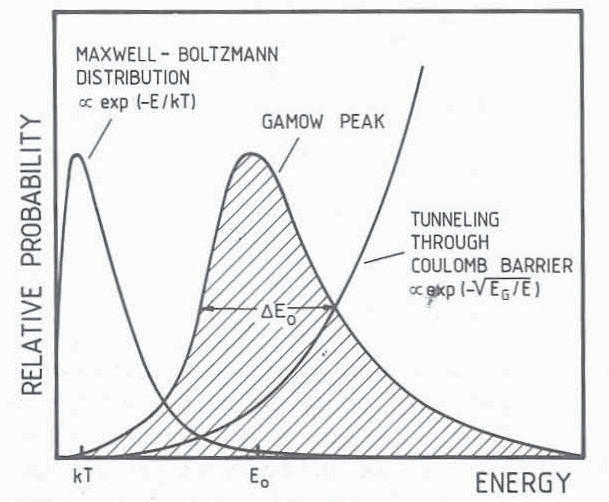
\includegraphics[scale=0.6]{graph/ch2/Gamow_window}}
    \caption{The schematic diagram of the Gamow peak. The hatched area is the product of Maxwell-Boltzmann distribution term and the  Coulomb penetrability term. $E_0$ shows the position of the maximum and $\Delta E_0$ indicates the Gamow window.}
    \label{fig:gamow_window}
  \end{center}
\end{figure}

The S-factor in the Gamow window can be considered as constant:
\begin{equation}
    \begin{aligned}
       S(E)=S(E_0)
    \end{aligned}
\end{equation}
Therefore, Eq.\ref{crosssection_S} reduces to
\begin{equation}
    \label{crosssection_S0}
    \begin{aligned}
     \langle\sigma v \rangle =(\frac{1}{\pi \mu})^{1/2} (\frac{1}{kT})^{3/2} S(E_0)\int_0^\infty  \exp(-\frac{E}{kT}-bE^{-1/2})dE
    \end{aligned}
\end{equation}

By calculating the maximum value of the integrand of Eq.\ref{crosssection_S0} one can get the effective burning energy
\begin{equation}
    \label{E_0}
    \begin{aligned}
       E_0=(\frac{bkT}{2})^{2/3}=1.22(Z_a^2 Z_A^2  \mu T_6^2)^{1/3}
    \end{aligned}
\end{equation}
where $\mu$ is in units of amu,  the stellar temperature $T_6$ is in units of $10^6$K and $E_0$  is in units of keV.

Substituting Eq.\ref{E_0} back into Eq.\ref{crosssection_S0}, one obtains the maximum of the reaction rate:
\begin{equation}
    \label{I_max}
    \begin{aligned}
        I_{max} = \exp(-\frac{3E_0}{kT})
    \end{aligned}
\end{equation}
and the exponential term in the integrand of Eq.\ref{crosssection_S0} can be approximated by a Gaussian function:
\begin{equation}
    \label{exp_gaus}
    \begin{aligned}
        \exp{(-\frac{E}{kT}-bE^{-1/2})} = I_{max}\exp[-(\frac{E-E_0}{\Delta /2})^2]
    \end{aligned}
\end{equation}
where $\Delta$ is the effective width of the energy window at  $1/e$ of the height of the Gamow peak and can be expressed by:
\begin{equation}
    \label{delta}
    \begin{aligned}
        \Delta = (4/3)^{1/2}(E_0kT)^{1/2}=0.749(z_a^2 Z_A^2 \mu T_6^5)^{1/6} \ keV
    \end{aligned}
\end{equation}


The energy region that contributes the most to the integrand falls into the Gamow window $(E_0\pm \Delta/2)$. Applying this approximation to Eq.\ref{exp_gaus}, the reaction rate becomes
\begin{equation}
    \label{crosssection_E0}
    \begin{aligned}
        \langle \sigma v \rangle  =  (\frac{2}{\mu})^{1/2} \frac{\Delta}{(kT)^{3/2}}S(E_0)\exp(-\frac{3E_0}{kT})
    \end{aligned}
\end{equation}



\subsection{Resonant Reaction Rates}

Unlike the one-step direct capture (nonresonant) reaction described above, the resonance reaction is a two-step process that is characterized by the strongly varying S-factor caused by a resonance. For an isolated resonance the cross-section is described by the Breit-Wigner formula (all quantities are in the center of mass system):
\begin{equation}
    \label{crosssection_BW}
    \begin{aligned}
        \sigma_{BW}(E) = \pi (\lambda/2\pi)^2 \frac{2J+1}{(2J_a+1)(2J_A+1)} \frac{\Gamma_a(E) \Gamma_b(E)}{(E-E_R)^2+(\Gamma(E)/2)^2}
    \end{aligned}
\end{equation}
where $\lambda$ is the de Broglie wavelength of the projectile defined by $\dfrac{\lambda^2}{2}=\dfrac{(\pi \hbar)^2}{\mu E}$, $E_R$ is the resonance energy and   $\Gamma_a(E)$, $\Gamma_b(E)$ and $\Gamma(E)$ are the energy-dependent partial widths of particle $a$, $b$ and the total resonance width, respectively. One can define the statistical factor  $\omega$ by the spins of the projectile $J_a$, target $J_A$ and resonant state $J$:
\begin{equation}
    \label{statistial_factor}
    \begin{aligned}
        \omega = \frac{2J+1}{(2J_a+1)(2J_A+1)}
    \end{aligned}
\end{equation}

Substituting Eq.\ref{crosssection_BW} and Eq.\ref{statistial_factor} into Eq.\ref{crosssection_1} the reaction rate per particle pair becomes:
\begin{equation}
    \label{crosssection_gamma}
    \begin{aligned}
        \langle \sigma v \rangle = \hbar^2 \omega \frac{\sqrt{2\pi}}{(\mu kT)^{3/2}} \int_0^\infty \frac{\Gamma_a(E) \Gamma_b(E)}{(E-E_R)^2 + (\Gamma(E)/2)^2} \exp(-E/kT)dE
    \end{aligned}
\end{equation}


If the partial width $\Gamma_i \ll E_R$, the resonance is considered to be narrow. In this case, the  Boltzmann factor $\exp(-E/kT)$ does not change significantly over the resonance region. Therefore, one can make the approximation that the partial widths and the exponential term in the integrand in Eq.\ref{crosssection_gamma} are independent of the energy $E$. Integrating Eq.\ref{crosssection_gamma} one gets
\begin{equation}
    \label{crosssection_width}
    \begin{aligned}
        \langle \sigma v \rangle = (\frac{2 \pi}{\mu k T})^{3/2} \hbar^2 (\omega \gamma)_R \exp(-E_R/kT)
    \end{aligned}
\end{equation}
where the width ratio is $\gamma = \Gamma_a\Gamma_b/\Gamma$. The strength of a resonance is defined by the product of these two terms $(\omega \gamma)_R$, as it refers to the integrated cross-section.


Eq.\ref{crosssection_width} is the stellar reaction rate per particle for a single narrow resonance. In the event of several narrow resonances, their contributions to the reaction rate are simply summed as
\begin{equation}
    \label{crosssection_sum}
    \begin{aligned}
        \langle \sigma v \rangle = (\frac{2 \pi}{\mu k T})^{3/2} \hbar^2 \sum_i(\omega \gamma)_i \exp(-E_i/kT)
    \end{aligned}
\end{equation}
or numerically, the reaction rate is given as
\begin{equation}
    \begin{aligned}
        N_A\langle \sigma v \rangle = 1.54\times10^5(\mu T_9)^{-3/2} \sum_i(\omega \gamma)_i \exp(-11.605E_i/T_9)
    \end{aligned}
\end{equation}
in units of cm$^{-3}$s$^{-1}$mol$^{-1}$. Here $T_9$ is the stellar temperature in units of $10^9$K, the resonance strength of the $i_{th}$ resonance $(\omega \gamma)_i$ and the $i_{th}$ resonate energy in the center of mass frame $E_i$ are in units of eV and MeV respectively.


\section{Indirect Measurement: Direct Reaction as a Spectroscopic Tool}

Many reaction rates of direct reactions involving charged particles are relevant for astrophysics at low energies where the Coulomb repulsion makes the cross-section very small and, therefore, extremely difficult to measure by  direct methods. Therefore, indirect methods are used to extract required information such as spectroscopic coefficients.

The Coulomb barrier can be associated with the penetrability which refers to the ability of particles that are trapped inside the potential barrier to tunnel through the barrier and escape from the nucleus. One can relate the partial widths  $\Gamma_{\lambda l}$ directly to the nuclear structure of the states of interest by treating the penetrability separately.

The wavefunction for a partial wave $l$ can be written as
\begin{equation}
    \label{wave_function}
    \begin{aligned}
        \Phi_{lm}(r,\theta, \varphi)=\frac{u_l(r)}{r} Y_{lm}(\theta, \varphi)
    \end{aligned}
\end{equation}
then the radial component of the solution of the Schrodinger equation for $u_l(r)$ becomes
\begin{equation}
    \label{ul}
    \begin{aligned}
        -\frac{\hbar^2}{2 \mu} \frac{d^2 u_l(r)}{dr^2} + [l(l+1)\frac{\hbar^2}{2\mu r^2}+ V(r) -E]u_l(r) =0
    \end{aligned}
\end{equation}
where the potential $V(r)$ has the form
\begin{equation}
    \label{Vr}
    V(r)=\left\{
    \begin{aligned}
    &V_{Coulomb} = z_1 Z_1 e^2/r, \ &r>R_n  \\
    &V_C + V_{nuc}, \  &r<R_n
    \end{aligned}
    \right.
\end{equation}
and $R_n$ refers to the radius of the nuclear part of the interaction potential between $a$ and $A$.

To relate the nuclear structure to the partial wave, one can assume that the actual wavefunction, in general, involves many configurations:
\begin{equation}
    \label{configuration}
    \begin{aligned}
    u_l = \sum_j \Theta_{ij} u_{lj}
    \end{aligned}
\end{equation}
where ${u_{ij}}$ could be the states in the particle-core coupling model. The coefficients $\Theta_{lj}$ ($0<\Theta_{lj}<1$) indicate the amplitudes of each of the configuration in the wavefunction. $\Theta^2_{lj}$ results in the probability of the configuration $u_{lj}$, as well as the probability of decay of each compound nuclear state to each state in the residual nucleus. In other words, they represent the spectroscopic strength of their specific wavefunction configuration. For example, in the particle-core coupling model, this  represents the decay to a continuum proton plus the core states indicated in $u_{ij}$. In some cases some of $u_{ij}$ might have the same core states. (For example, a $d_{3/2}$, $d_{5/2}$ and $s_{1/2}$ neutron coupled to a $2^+$ core state could form $J^{\pi}$ = 3/2${^+}$ or 5/2$^{+}$ states.) Then all such states could decay to that core state. This approach does allow us to develop a relationship between the width of the state $\Gamma_{lj}$ and the coefficients in the wavefunction, the $\Theta{ij}$
\begin{equation}
    \label{spectroscopic_relation}
    \begin{aligned}
    \Gamma_p = C^2S \Gamma_{sp}
    \end{aligned}
\end{equation}
where $\Gamma_{sp}$ denotes the partial width of a single-particle resonance located at the same energy as the resonance of interest. $C$ is the Clebsch-Gordan coefficient.


Typically the spectroscopic factor $S$ are extracted in transfer reactions by a comparison of experimental cross-sections and the result of DWBA calculations by appropriately choosing the optical-model potential. Considering a transfer reaction A$+$c $\rightarrow$ B$+$b (c$=$a$+$b), the reaction process can be divided into two steps. Firstly, particle c breaks up into a and b near the core A (c$\rightarrow$ a$+$b). Secondly, a is captured by core A thus generates core B (a$+$A $\rightarrow$ B), as  shown schematically in Fig.~\ref{fig:transfer}

The transfer reaction A$+$c$\rightarrow$ B$+$b is composed by the capture reaction a$+$A $\rightarrow$ B$+$b and the inverse process a$+$b $\rightarrow$ c$+$$\gamma$. Therefore, the cross-section should be associated with  two spectroscopic factors $S_{ab}$ and $S_{Aa}$ by
\begin{equation}
    \label{transfer_crosssection}
    \begin{aligned}
    \sigma  = \sum_{j_B j_c} S_{A a l_B j_B} S_{a b l_c j_c} \sigma^{DWBA}_{l_B j_B l_c j_c}
    \end{aligned}
\end{equation}
 where $\sigma^{DWBA}_{l_B j_B l_c j_c}$ is the cross-section calculated by DWBA. By experimentally measuring the cross-sections of the transfer reaction $A+c \rightarrow B+b$ and theoretically  calculating $\sigma^{DWBA}_{l_B j_B l_c j_c}$,  the  spectroscopic  factor $S_{Aa}$ can be obtained if $S_{ab}$ is known.

\begin{figure}[tpb]
  \begin{center}
    \centerline{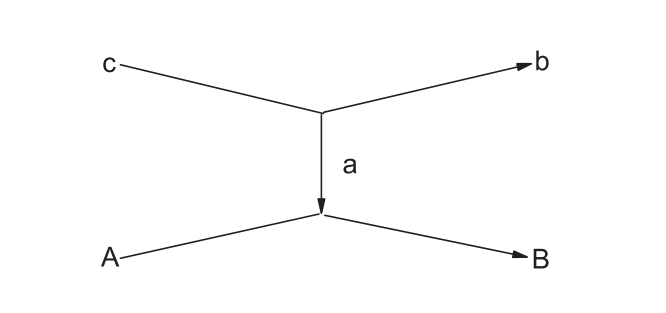
\includegraphics[scale=0.6]{graph/ch2/transfer}}
    \caption{The process of the transfer reaction  $A+c \rightarrow B+b$}
    \label{fig:transfer}
  \end{center}
\end{figure}

 As  mentioned above, $S_{Aa}$ is sensitive to the optical model potentials. However, in terms of particle widths of unbound states, it is shown that the experimentally measured particle width $\Gamma_p$ does not critically depend on the selected potential. This is a consequence of the fact that $\Gamma_{sp}$ also depends on the potential resulting from Eq.~\ref{spectroscopic_relation}. This cancels most of the potential dependence as long as both values are extracted with the same potential.  Thus the particle width can be determined in the same theoretical framework in which the spectroscopic factor is determined.




% To subtract the spectroscopic factor $S$, $\Gamma_p$ is obtained by the experimental data and $\Gamma_{sp}$ can be computed numerically by solving Schrodinger equation for the elastic scattering


% The spectroscopic factor is a tool to get the cross section of the direct measurement.
% \begin{equation}
%     \begin{aligned}
%         \sigma = \lambda \dot |M|^2
%     \end{aligned}
% \end{equation}
% where $\lambda$ is the kinematic factor, $M$ is the transition amplitude of the reaction,
% \begin{equation}
%     \begin{aligned}
%         M=\langle \varphi_B(\zeta_A,\zeta_a,\textbf{r})|\hat{O}(\textbf{r})|\varphi_A(\zeta_A)\zeta_a (\xi_a)\phi^{(+)}_{k_i}(\textbf{r}) \rangle
%     \end{aligned}
% \end{equation}
% where $\varphi_i$, $\zeta_i$ are the wave function of the bound state and the intrinsic coordinates
%  the nuclei $i$, respectively; $\textbf{r}$ is the relative distance between $a$ and $A$; $\hat{O}$ is the electronic transition operator; $\phi^{(+)}_{k_i}$ is the wave function of the incoming wave. Integral to the intrinsic coordinate to get the stacked wave function.
%  \begin{equation}
%     \begin{aligned}
%         I_{Aa}^B(\textbf{r}) = (A+a)^{1/2}\langle\varphi_A(\zeta_A)\varphi_a(\zeta_a)|\varphi_B(\zeta_A, \zeta_a,\textbf{r})\rangle
%     \end{aligned}
% \end{equation}

% The physics meaning of $I_{Aa}^B(\textbf{r})$ is the wave function of the bound state of $B=A+a$  $\varphi_B$ , project to

%  \begin{equation}
%     \begin{aligned}
%         M=\langle I_{Aa}^b(\textbf{r})|\hat{O}| \phi^{(+)}_{k_i}(\textbf{r}) \rangle
%     \end{aligned}
% \end{equation}

%  $I_{Aa}^b(\textbf{r})$ is not the bound state B.

%   \begin{equation}
%     \begin{aligned}
%         S_{Aa}^B = \int_{0}^{\infty} (I_{Aa}^B(\textbf{r}))^2 d{\textbf{r}}
%     \end{aligned}
% \end{equation}

% is the spectroscopic factor.
% \begin{equation}
%     \begin{aligned}
%         I_{Aa}^B(\textbf{r}) =& (A+a)^{1/2} \langle \varphi_A(\zeta_A) \varphi_B(\zeta_A, \zeta_a, \textbf{r})\rangle \\
%                              =& \sum_{l_B m_{l_B} j_B m_{j_B}} \langle J_A M_A j_B m_{jB}|J_B M_B \rangle \\
%                               &\times \langle J_a M_a l_B m_{j_B}|j_B m_{l_B}\rangle i^{l_B} Y_{l_B m_B}(\hat{\textbf{r}}) I^B_{Aal_B J_B}(r)
%     \end{aligned}
% \end{equation}

% where $J_i$, $M_i$ is the spin and projection of the nuclei $i$, $\langle J_a M_a l_B m_{l_B} | j_B m_{j_B}\rangle$ is the C-G coefficient, $Y_{l_B m_B}(\hat{\textbf{r}})$ is the Spherical Harmonic Function, $I^B_{Aal_BJ_B}(r)$ is the radius integral of the dieji wave function.

% In the model of the single particle, the dieji wave function $I^B_{Aal_BJ_B}(r)$ can be considered as the production of the spectroscopic factor and the bound state wave function of the particle.

%   \begin{equation}
%     \begin{aligned}
%         I^B_{Aal_BJ_B(r)} \approx (S_{l_B j_B})^{1/2} \varphi_{n_B l_B j_B}(r)
%     \end{aligned}
% \end{equation}
% where  $\varphi_{n_B l_B j_B}(r)$ is the normalized jingxiang  wave function of $B=A+a$, which can be solve from the bound state Schrodinger function. As a  result, calculating the $ I^B_{Aal_BJ_B}(r)$ became calculating the spectroscopic factor $S_{l_B j_B}$.

% The spectroscopic factor can be obtained by calculating the cross section of the transferred reaction. For the transfer reaction $A+c \rightarrow B+b(c=a+b)$ the reaction can be considered as two steps: The first step is the breakup of $c$ to $a$ and $b$ near core $A$ ($c \rightarrow a+b$). The second step is $a$ is captured by core $A$ and produce $B$ ($a+A \rightarrow B$).


% The transfer reaction $A+c \rightarrow B+b$ can be considered as the radiation capture reaction $a+A \rightarrow B+\gamma$ and the inverse process $a+b \rightarrow c + \gamma$.








% % uncomment the following lines,
% if using chapter-wise bibliography
%
% \bibliographystyle{ndnatbib}
% \bibliography{example}
